\documentclass[12pt]{report}
\usepackage{amsmath}
\usepackage{amssymb}
\usepackage{graphicx}
\graphicspath{ {images/} }
\usepackage[headheight = 50pt, top=1.5in, bottom=1in, left=1in, right=1in]{geometry}
\usepackage{fancyhdr}

\pagenumbering{gobble}
\pagestyle{fancy}

\newcommand{\norm}[1]{\left\lVert #1 \right\rVert}
\renewcommand{\headrulewidth}{4pt}
\lhead{
Class: Deep RL\\
SID: 24274554\\
Name: Varun Tolani
\\
HW: 1\\
}
\fancyhead[R]{\sf\rightmark}
\begin{document}
\section*{Behavioral Cloning}
\subsection*{1.}
For both the Ant and Reacher tasks I trained a neural network with 3 hidden layers with relu activations. The Ant network has layers size 111-64-64-32-8 and the Reacher network 11-10-10-7-2 (in order). The loss used in both networks was:
\begin{center}
$L=\sum \norm{a_{expert}-a_{pred}}_2 + \alpha \norm{W}_2$
\end{center}
Here we aim to minimize the eculidean distance between our predicted actions and the expert actions with an additional l2 penalty on the weights of the network to prevent overfitting. The $\alpha$ hyperparameter was chosen via cross validation and is $10^{-5}$ for the Ant network and $10^{-4}$ for the Reacher network.\\ \\
Both networks were trained using SGD with mini batches of size 50 for 500 gradient steps. The learning rate for both was $10^{-3}$ and was chosen via cross validation.\\
\\
I generated 20 rollouts for the Ant environment and 400 rollouts for the Reacher environment for a total of 20000 samples each.\\
\newpage
\begin{center}
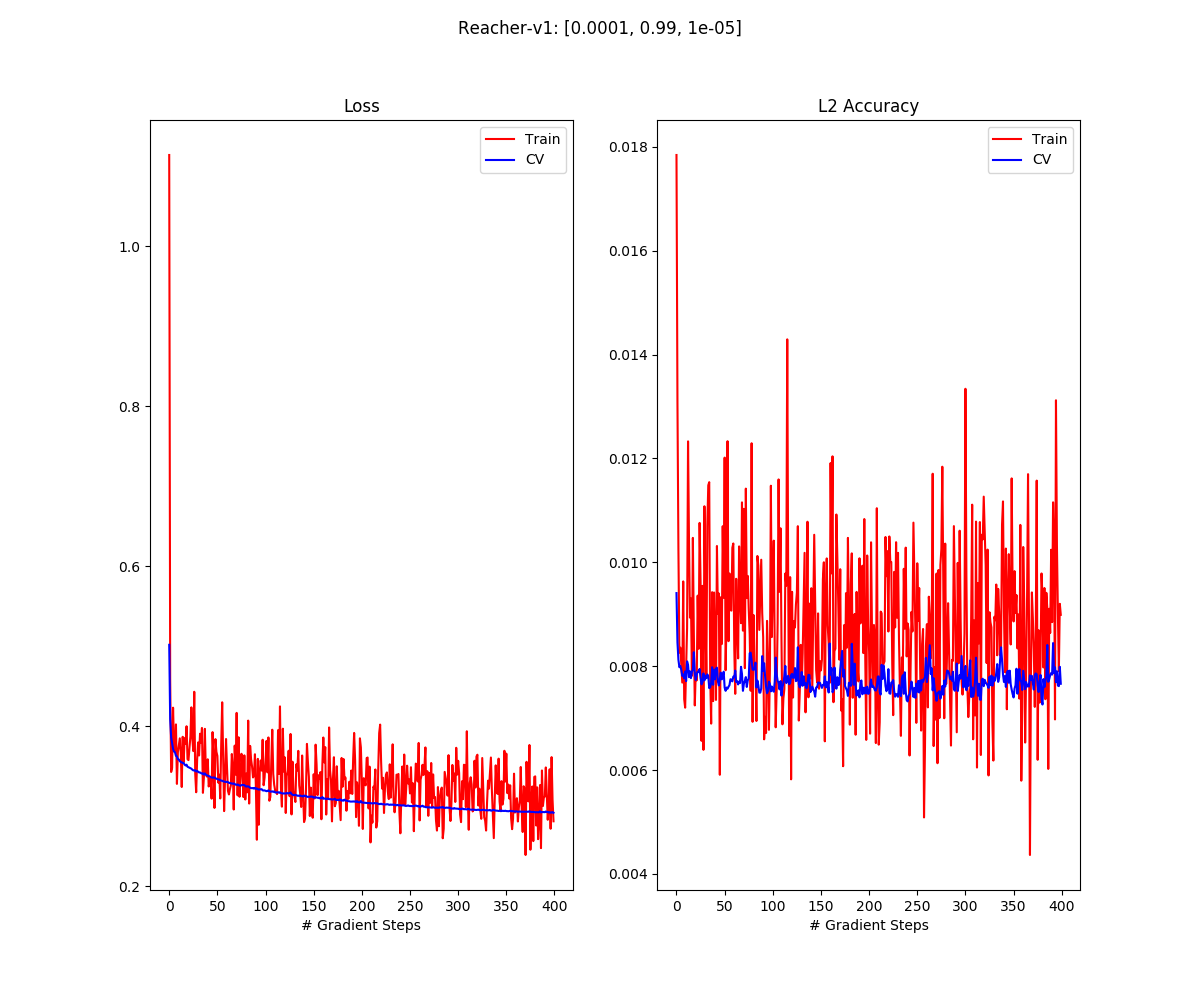
\includegraphics[scale=.6]{./images/reacher_train_summary.png}
\end{center}
For the Reacher environment over 400 rollouts (20,000 samples) the behavioral cloning agent recieved:\\
$\mathbb{E}[r]=-11.81$\\
$\sigma(r) =  5.25$\\
\\
The expert policy over 20 rollouts received:\\
$\mathbb{E}[r]=-3.9318$\\
$\sigma(r) =  1.617$\\
\newpage
\begin{center}
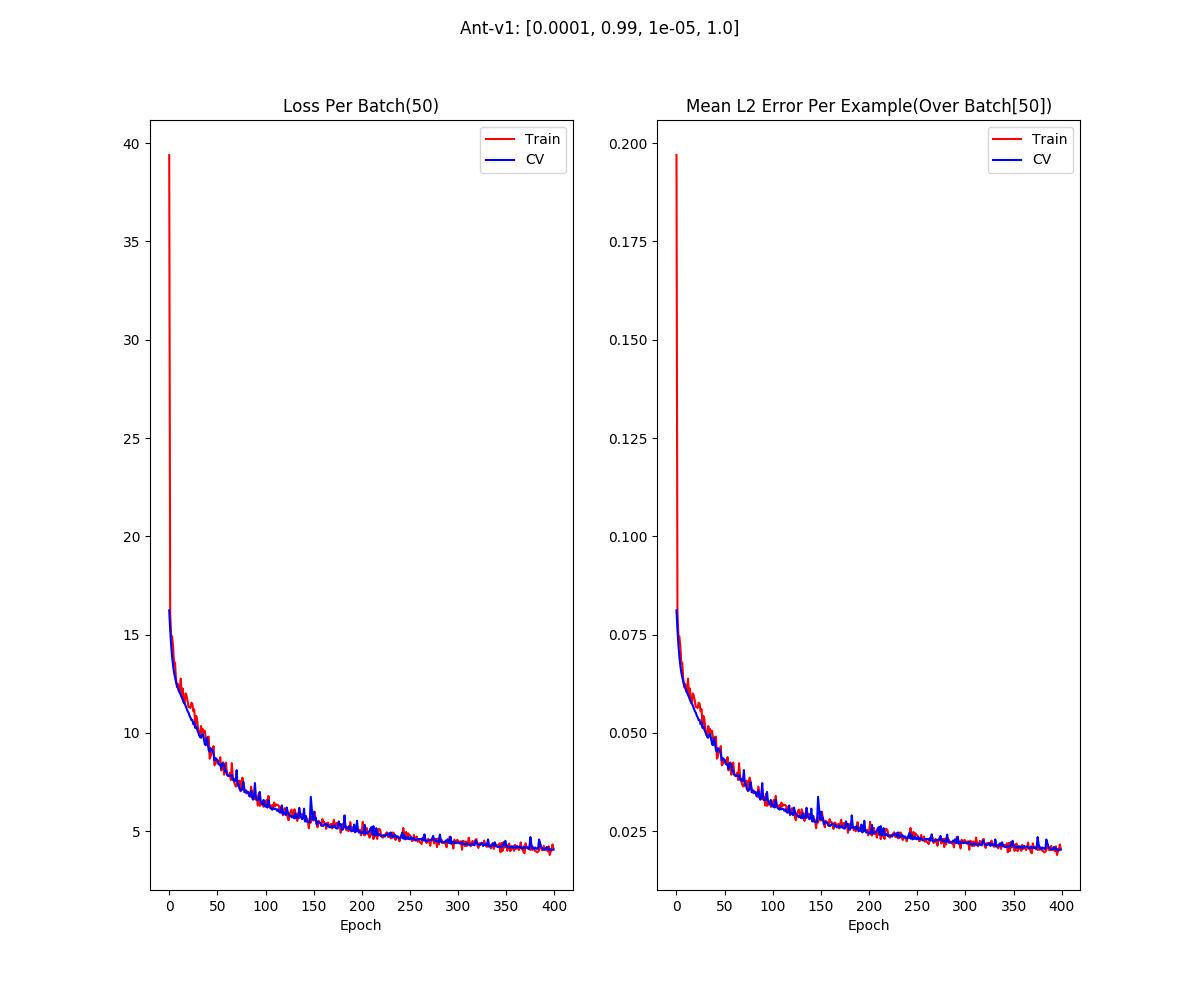
\includegraphics[scale=.6]{./images/ant_train_summary.png}
\end{center}
For the Ant environment over 20 rollouts (20,000 samples) the behavioral cloning agent received:\\
$\mathbb{E}[r]=1178.75$\\
$\sigma(r) =   82.1$\\
\\
The expert policy over 20 rollouts received:\\
$\mathbb{E}[r]=4814.742$\\
$\sigma(r) =   78.722$\\
\subsection*{2}
I decided to test dropout on my behavioral cloning model for the Reacher environment. The model architecture is 3 fully connected layers size 10, 10, 7 (with relu activations) as well as an input layer  size 11 and an output layer size 2. Between the last fully connected layer and the output sits a dropout layer with tuneable probability of dropout. I varied the keep propability (1-dropout probability) in increments of .025 from .7 to 1 and plotted the change in mean and standard deviation on the Reacher task across 400 rollouts.
\begin{center}
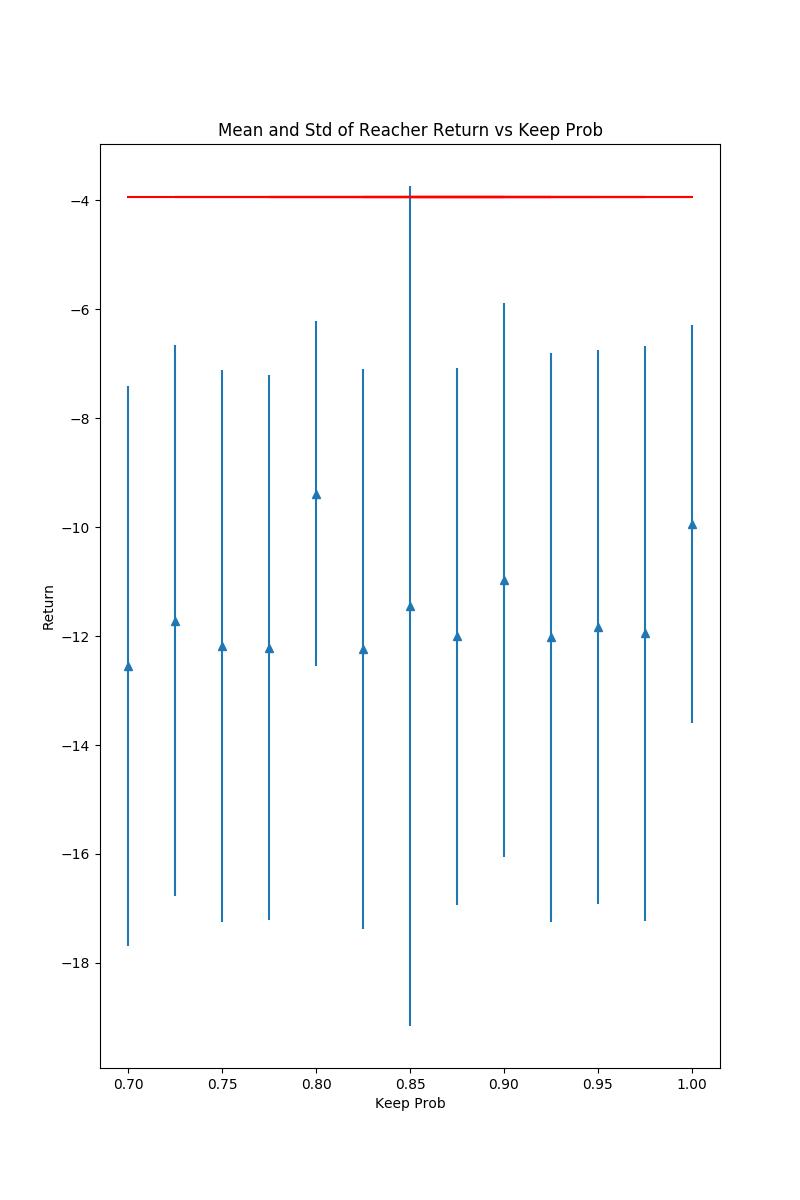
\includegraphics[scale=.5]{./images/2_2.png}
\end{center}
\vspace*{.5in}
As stated earlier, for the Reacher environment over 400 rollouts the expert policy recieved:\\
The expert policy over 400 rollouts received:\\
$\mathbb{E}[r]=-3.9318$\\
$\sigma(r) =  1.617$\\

Keep probability of 1.0 achieved results closest to the expert policy so I decided to use 1.0 (no dropout) for this hyperparameter.
\newpage
\section*{DAgger}
\begin{center}
\includegraphics[scale=.75]{dagger_training.png}
\end{center}

As can be seen above the DAgger algorithm converges to the expert policy behavior farily quickly. It does not achieve the same mean return on the Reacher task but it does do better than standard BC (iteration 1). To see the effects of DAgger I had to shrink the size of my NN used to represent the BC policy. For simple tasks such as Reacher the expressiveness of my previous NN model already did so well that dagger hardly had any noticeable improvements. My final model for the Reacher task has one hidden layer with size 10 as well as input and output layers while my previous Reacher model had 3 hidden layers.\\
\\
I initialized my agent by running behavioral cloning for 5 epochs (20 batches of size 50 each) on 20000 examples from the expert policy. In each iteration of the DAgger algorithm I then ran 10 rollouts, generating 10,000 more examples, and appended these to the dataset. For each subsequent iteration of DAgger I train an entirely new model on the aggregated dataset- training for 5 epochs each iteration.

\end{document}